\section{Downstream Biological Utility}
\label{sec:downstream}

\subsection{Marker Recovery}

For each dataset and split seed $s\in\{11,23,37,53,71\}$, we stratify cells into
50\% reference and 50\% evaluation subsets.  Reference markers are the top 100
Wilcoxon-ranked genes for each true type using reference cells only.  Evaluation
markers are independently ranked for each predicted cluster; true evaluation
labels do not enter differential expression.  Type--cluster overlap matrices
yield Recovery@20, @50, and @100, Jaccard similarity, overlap coefficient, and
the fraction of evaluation clusters without at least three valid markers.
Unmatched reference types contribute zero to recovery rather than disappearing
from the mean.

\subsection{Marker-Overlap Annotation}

Each predicted cluster is assigned the reference type with maximum marker
overlap; multiple clusters may map to the same type.  Ties are resolved by mean
shared-marker log fold change and then lexicographically.  A cluster with fewer
than three markers or zero maximum overlap is \texttt{unassigned}.  Evaluation
cells are scored by accuracy, balanced accuracy, macro-F1, per-class recall, and
coverage.  Hungarian mapping is reported only as an oracle upper bound and is
never described as a practical annotation method.

\subsection{Low-Label Frozen-Embedding Probe}

At 10\% and 30\% label fractions, a stratified subset trains
\texttt{StandardScaler} followed by L2 multinomial logistic regression
($C=1$, balanced class weights, 2,000 maximum iterations).  The scaler and
classifier are fit only on the training subset; the encoder remains frozen.
We report accuracy, balanced accuracy, macro-F1, and per-class recall over the
five fixed split seeds.  This is within-dataset transductive annotation and does
not establish cross-dataset transfer.

\subsection{Human Pancreas 3 Case Study}

The case study fixes scMAE/NoMix, scVICAR-F, and scVICAR-T before inspecting
markers.  It combines a marker dot or track plot, type--cluster overlap heatmap,
and a reference-type $\rightarrow$ predicted-cluster $\rightarrow$ marker
annotation $\rightarrow$ gold-type Sankey diagram.  A literature-verified
pancreatic marker panel is used only for interpretation.  It is neither a
training input nor a model-selection criterion.  The panel is frozen from the
primary human-pancreas atlas literature, principally Baron et
al.~cite{baron2016pancreas,segerstolpe2016pancreas}.  We distinguish the 8,629
human cells reported after quality control in the primary Baron article, the
8,569-cell benchmark input, and the 8,562 cells retained by our prespecified
filter; these numbers describe different processing stages rather than a
discrepancy in the confirmatory analysis.  Figure~\ref{fig:pancreas-case}
reports the fixed case without selecting a favorable seed or split.

\begin{figure*}[t]
  \centering
  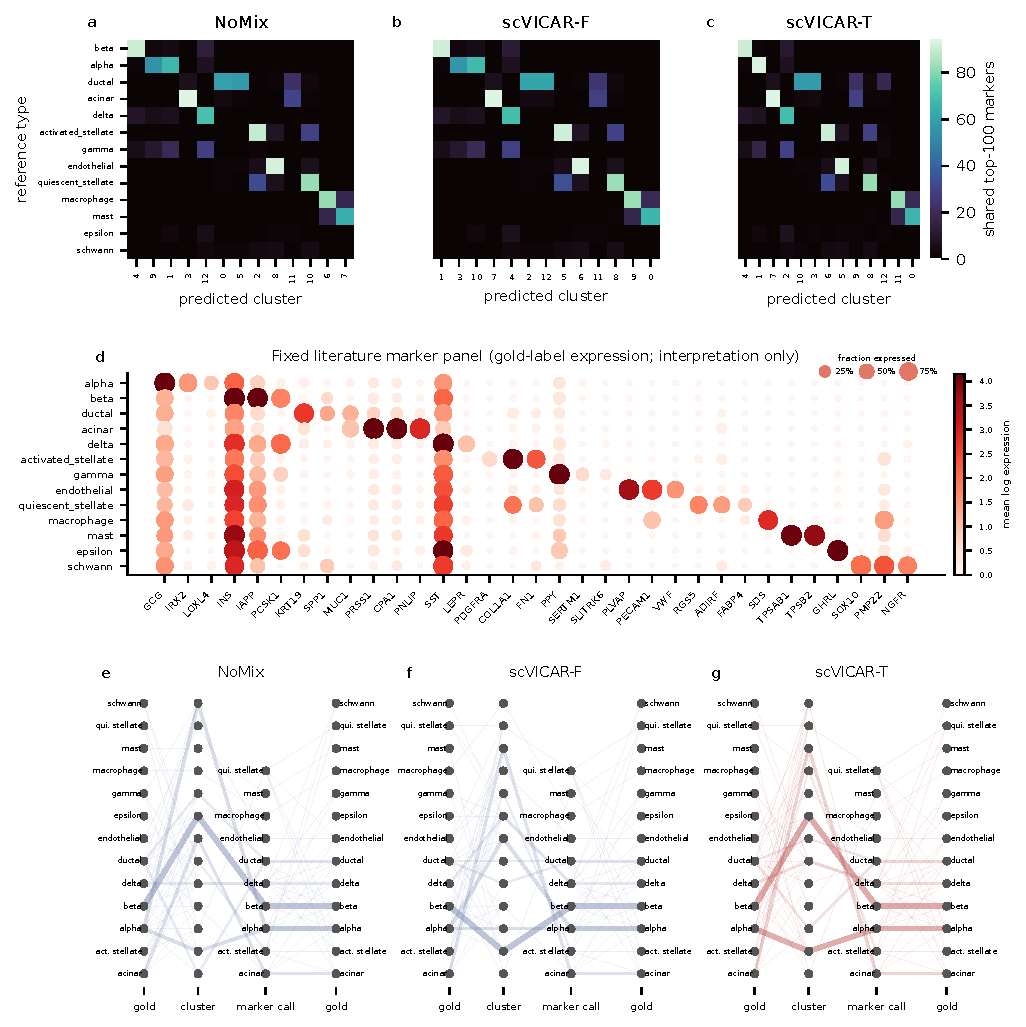
\includegraphics[width=\textwidth]{../figures/final/fig6_pancreas_case.pdf}
  \caption{Preregistered Human Pancreas 3 case study (model seed 42, downstream
  split seed 11). (a--c) Reference-marker overlap by predicted cluster for
  NoMix, scVICAR-F, and scVICAR-T. (d) Expression prevalence and mean normalized
  expression of a literature-verified pancreas marker panel, shown for
  interpretation only. (e--g) Reference type $\rightarrow$ cluster
  $\rightarrow$ marker-overlap annotation $\rightarrow$ held-out gold type.
  Line width represents cell count; the marker panel is not used for training,
  graph construction, or model selection.}
  \label{fig:pancreas-case}
\end{figure*}
\clearpage

All downstream computations reuse remotely archived embeddings and write their
split-level outputs under the originating run identifier.  Results are reported
completely even when they do not support an advantage, in which case the claim
is narrowed to representation geometry or clustering as appropriate.

% Replaced only after all downstream run IDs pass checksum and completeness QA.

